\documentclass{article}
\usepackage{times}
\usepackage{mcode}
\usepackage{graphicx}
\usepackage{caption}
\usepackage{subcaption}
\usepackage{mathtools}
\usepackage{enumerate}

\begin{document}
\title{Image Processing Exercise Book, TDT4195}
\author{Olav Olseng}
\maketitle
\newpage


\section{Exercise 1}
\subsection{Basic Image Processing}
\subsubsection*{Task 1}
I first read the images converting to doubles by typing into the "img" and "flatField" variables. I then use the imdivide function from the images toolbox to get a pixel-by-pixel division, and I store the result in my "res" variable. To show the result, i use the imshow function.

\begin{lstlisting}	
	img = im2double(imread('testimages/disturbed_potw1144a.png'))
	flatField = im2double(imread('testimages/flatfieldimage.png'))
	res = imdivide(img, flatField)
	imshow(res)
\end{lstlisting}
The images are loaded and normalized in a clamped double (values are between 0.0 and 1.0), with this loading function.
The finalized images look like this:
\\
\begin{figure}[h]
	\centering
	\begin{subfigure}[b]{0.45\textwidth}
		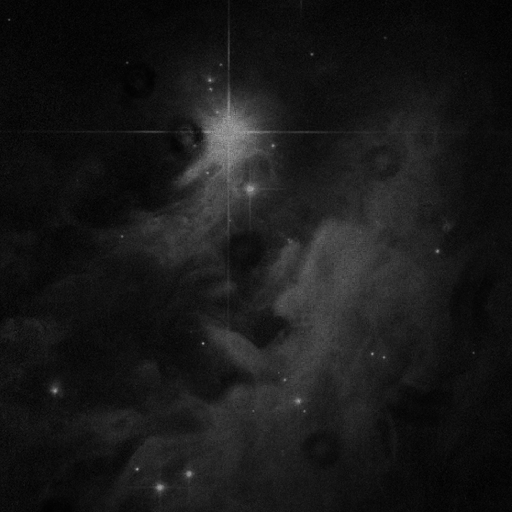
\includegraphics[width = \textwidth]{astro1.png}
		\caption{Original image}
		\label{fig:astro1.png}
	\end{subfigure}
	\begin{subfigure}[b]{ 0.45\textwidth}
		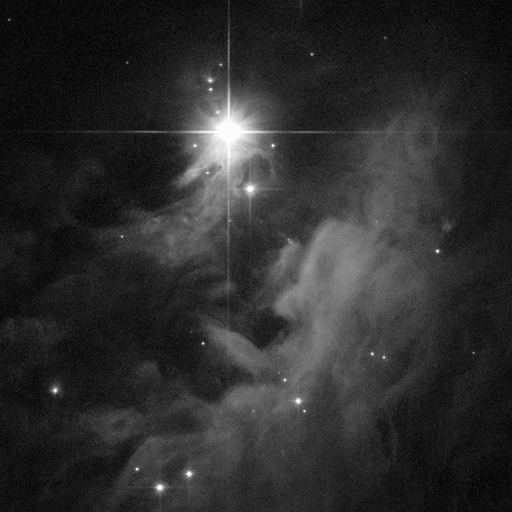
\includegraphics[width=\textwidth]{astro2.png}
		\caption{Processed image}
		\label{fig:astro2.png}
	\end{subfigure}
\end{figure}
\subsubsection*{Task 2}
We use division to \emph{increase} the gray-level, if we subract it becomes darker. This is due to the fact that the images are normalized withing [0.0, 1.0]. So the blacker the value of the flatfield image is, the brighter the result image will be in that particular pixel. This can however, create problems if the flatfield image has pixel values of 0 (completely black), as we might get division by zero.


\newpage
\subsection{Filtering}
\subsubsection*{Task 1}
The image in the task is, at the time of writing, 17 pixels wide, not 16.\\ Original image:
\\
\begin{tabular}{|c|c|c|c|c|c|c|c|c|c|c|c|c|c|c|c|c|}
	\hline
	0 & 0 & 0 & 0 & 0 & 0 & 1 & 1 & 1 & 1 & 1 & 0 & 0 & 0 & 0 & 0 & 0 \\ 
	\hline
\end{tabular}
\paragraph{(a)}
The result i get from applying the filter to the 1D image is this:
\\
\begin{tabular}{|c|c|c|c|c|c|c|l|c|c|c|c|c|c|c|c|c|}
	\hline
	  &   & 0 & 0 & 1 & 2 & 3 & 4 & 5 & 4 & 3 & 2 & 1 & 0 & 0 &   &   \\ 
	\hline
\end{tabular}

\paragraph{(b)}
There isn't any need to apply extra padding in this example, it already seems to be padded with the six 0s on each side of the five 1s in the original image. So there isn't any real loss of data. This really depends on the implementation of the filter however.

\subsubsection*{Task 2}
If we do apply the continious convulution of this function we end up with:

\paragraph{(a)}
\begin{equation}
	\int_{-1/2}^{1/2} 1 \times 1 {d}v = 1
\end{equation}

\paragraph{(b)}
I expect this to give a the shape of a podium. Like they have in the olympics.

\newpage
\subsection{Noise}
\subsubsection*{Task 1}

I chose the mandrill picture for this assignment. I applied the different salt \& pepper noise densities of 0.1, 0.3 and 0.5. \\
The noise was applied using the images toolbox function suggested in the assignment.
\begin{lstlisting}
	P = imnoise(I, 'salt & pepper', 0.1)
\end{lstlisting}

\begin{figure}[h]
	\centering
	\caption {Different salt and pepper noise densities}
	\begin{subfigure}[b]{0.3\textwidth}
		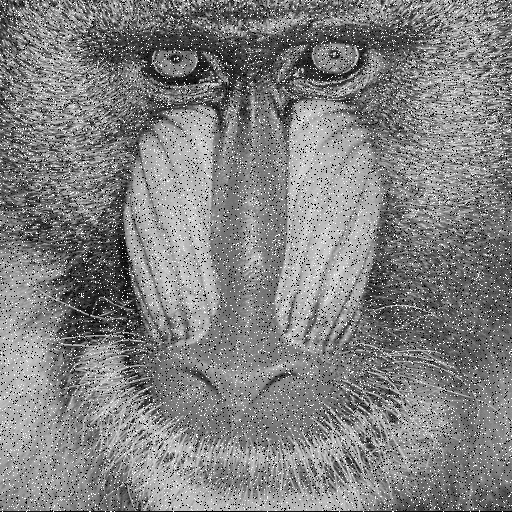
\includegraphics[width = \textwidth]{Mandrill01.png}
		\caption{0.1 Density}
		\label{fig:Mandrill01.png}
	\end{subfigure}
	\begin{subfigure}[b]{0.3\textwidth}
		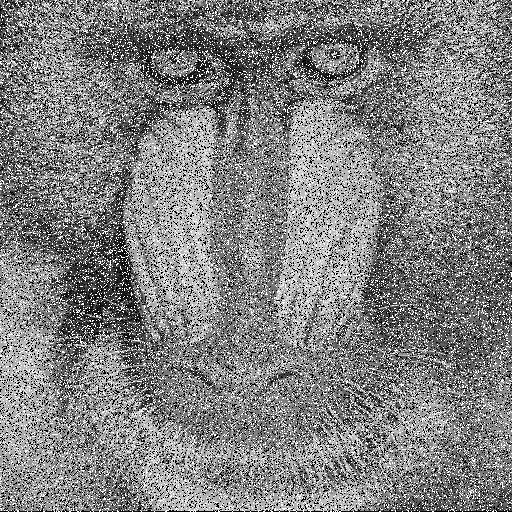
\includegraphics[width = \textwidth]{Mandrill03.png}
		\caption{0.3 Density}
		\label{fig:Mandrill03.png}
	\end{subfigure}
	\begin{subfigure}[b]{0.3\textwidth}
		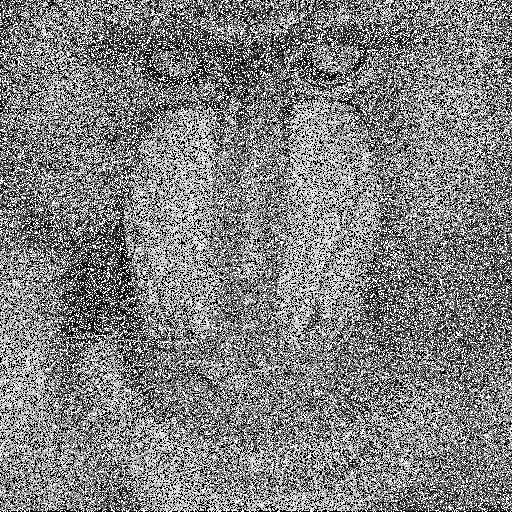
\includegraphics[width = \textwidth]{Mandrill05.png}
		\caption{0.5 Density}
		\label {fig:Mandrill05.png}
	\end{subfigure}
\end{figure}

Other noise types include, but not limited to, gaussian noise, uniform noise and exponential noise.

\newpage
\subsection{Aliasing}
\subsubsection*{Task 1}
Here are the brick images with different sampling rates:\\

\begin{figure}[h]
	\centering
	\begin{subfigure}[t]{0.49\textwidth}
		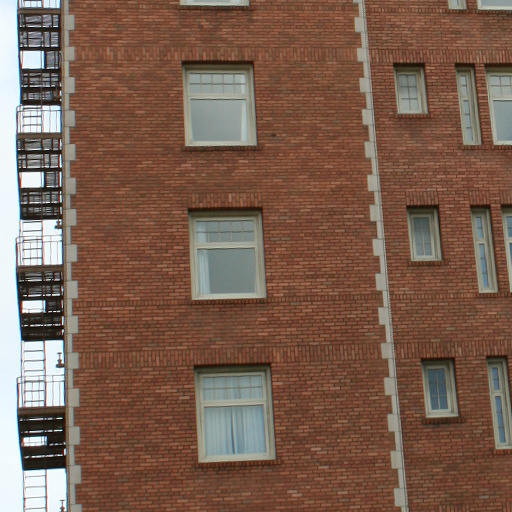
\includegraphics[width = \textwidth]{aliasbrick1.png}
		\caption{Original image}
		\label{fig:aliasbrick1.png}
	\end{subfigure}
	\begin{subfigure}[t]{0.49\textwidth}
		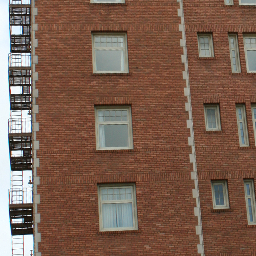
\includegraphics[width = \textwidth]{aliasbrick2.png}
		\caption{Half of image sampled}
		\label{fig:aliasbrick2.png}
	\end{subfigure}
	\begin{subfigure}[b]{0.49\textwidth}
		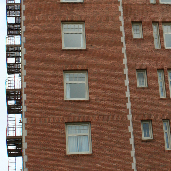
\includegraphics[width = \textwidth]{aliasbrick3.png}
		\caption{Third of image sampled}
		\label{fig:aliasbrick3.png}
	\end{subfigure}
	\begin{subfigure}[b]{0.49\textwidth}
		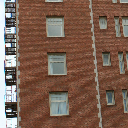
\includegraphics[width = \textwidth]{aliasbrick4.png}
		\caption{Fourth of  image sampled}
		\label{fig:aliasbrick4.png}
	\end{subfigure}
\end{figure}

As there is a pattern in the way the bricks a distributed in the wall, this pattern gets malformed as we downsample the image. Especially when we keep only a third and a fourth of the original data, we see new patterns emerge at the bottom of the wall.
This effect was not as prevalent when i did the same downsampling on the lena.png image. This might be due to the fact that the image of a woman, doesn't have such a mathematical pattern in it, as the brickwall does.

\newpage
\section{Exercise 2}
\subsection{Point Processing}
\subsubsection*{Intensity Transform}

The original image of Einstein has a fairly low contrast, and we want to change it. \\
\begin{figure}[h!]
	\centering
	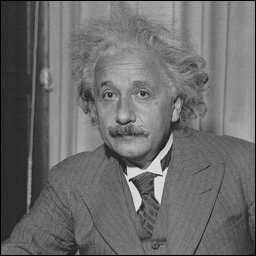
\includegraphics[width = 0.35\textwidth]{einstein.png}
	\caption{Original Image}
\end{figure}
\\
Using the standard built in imadjust function in MatLab, the yielded result is this:\\
\begin{figure}[ht!]
	\centering
	\includegraphics[width = 0.35\textwidth]{einsteinStock.png}
	\caption{The default gammatransform in MatLab}
\end{figure}

It turns out that my version of MatLab calls the stretchlim() finction as an input value by default, and yielded the same results as above. The intensity values range from 0 : 255 in both images.

\newpage
\subsection{Histogram Equalization}
\paragraph{1.}
A histogram will not be completely uniform after a histogram equalization, because all the pixels with the same intensity value \emph{X} before the transformation should have the same intensity value \emph{Y} after the transformation. If we do not not retain this relationship through the transformation, it would be like changing pixels that had the same colour before a transformation, into different colors after the transformation. It would ruin our perception of the image. 

\paragraph{2.}
You can tell that an image has a low contrast on it by looking at how the histogram is distributed. If the min-max intensity values are close, it means that the image does noe utilise the entire dynamic range we have at our disposal. Meaning a low contrast. The original einstein photo from task 1 has intensity value in the range [0.29 : 0.70], meaning it only utilises 40\% of the dynamic range that i could have.

\paragraph{3.}
I wrote a MatLab function for this. It goes as follows:
\begin{lstlisting}
function res = histogramEQ(image, dynamicRange)
    %setup variables
    [x, y] = size(image);
    pixels = x * y;
    hist = zeros(dynamicRange + 1, 1);
    
    %calculate and normalize the histogram
    for i = (0:dynamicRange)
        hist(i + 1) = sum(sum(image == i));
    end
    
    %calculate cumulative distribution
    current = 0;
    cum = zeros(length(hist), 1);
    for i = (1:length(cum))
        current = current + hist(i);
        cum(i) = current;
    end
    cum
    cum = cum / pixels;
    %make blank result image
    res = zeros(size(image));
    
    %map new values from original into res
    for row = (1:size(image, 1))
        for col = (1:size(image, 2))
            res(row, col) = cum(image(row, col) + 1);
        end
    end
\end{lstlisting}

\newpage
\paragraph{4.}
The result I got from my function was only slightly off from the built in MatLab function, given that I supplied the dynamic range of 256 to my algorithm. Mine had a bit more whitenoise. You can barely see it under the upper right bookshelf:
\begin{figure}[ht!]
	\centering
	\begin{subfigure}[t]{0.49\textwidth}
		\includegraphics[width = \textwidth]{myeinstein.png}
		\caption{My function}
		\label{fig:myeinstein.png}
	\end{subfigure}
	\begin{subfigure}[t]{0.49\textwidth}
		\includegraphics[width = \textwidth]{MLeinstein.png}
		\caption{histeq() function}
		\label{fig:MLeinstein.png}
	\end{subfigure}
\end{figure}
\\
The results are quite terrible. This is due to the fact that the contrast in the image is so low, the slightly brighter pixels get set to white if they are over a certain threshold.
\\
Applying my function to the mandrill from exercise one, the results are much better. This is due to the higher contrast range in the raw image.
\begin{figure}[ht!]
	\centering
	\begin{subfigure}[t]{0.49\textwidth}
		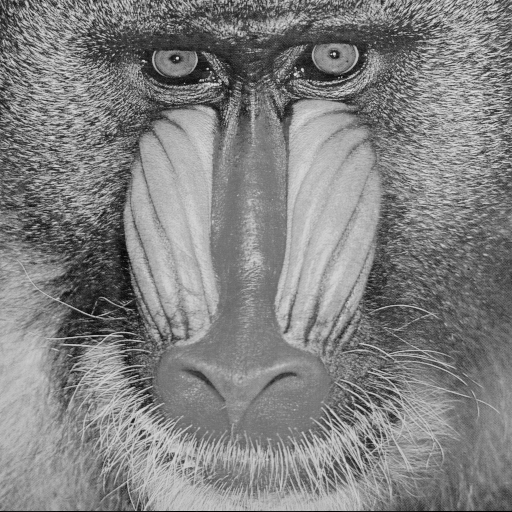
\includegraphics[width = \textwidth]{mandrill.png}
		\caption{Origianl mandrill}
		\label{fig:mandrill.png}
	\end{subfigure}
	\begin{subfigure}[t]{0.49\textwidth}
		\includegraphics[width = \textwidth]{mymandrill.png}
		\caption{My mandrill}
		\label{fig:mymandrill.png}
	\end{subfigure}
\end{figure}

\subsection{Pixel Connectivity}
\begin{enumerate}[(a)]
	\item There are 3 4-connected components in S1, and 3 in S2.
	\item There are 5 8-connected components in S1, and 5 in S2.
	\item If we use 8-neighbourhoud, S1 and S2 are connected, as we have a diagonal between S2(1, 3) and S1(4, 4).
\end{enumerate}

\subsection{Spatial Filtering}
I designed and exported the two images as suggested, yielding the result:
\begin{figure}[h]
	\centering
	\begin{subfigure}[b]{0.45\textwidth}
		\includegraphics[width = \textwidth]{sp25man.png}
		\label{fig:sp25man.png}
		\caption{Salt \& pepper noise}
	\end{subfigure}
	\begin{subfigure}[b]{0.45\textwidth}
		\includegraphics[width = \textwidth]{gau01man.png}
		\label{fig:gau01man.png}
		\caption{Gaussian noise}
	\end{subfigure}
\end{figure}

\newpage
For solving the next two parts I wrote a spatial filter function taking in the parameters: image, filtersize and the filtertype. It is written as follows:

\begin{lstlisting}
function res = spatFilter(image, filtersize, type)
    res = zeros(size(image, 1) , size(image, 2));
    filtermid = uint8(filtersize/2);
    filterborder = filtermid - 1;
    
    for i = filtermid:(size(image, 1) - filterborder)
        for j = filtermid:(size(image, 2) - filterborder)
            %calculate bounds
            leftBound = i - filterborder;
            rightBound = i + filterborder;
            upBound = j - filterborder;
            downBound = j + filterborder;
            %slice out filtersample
            sample = image(leftBound:rightBound, upBound:downBound);
            
            pixelval = 0;
            if (type == 'avg')
                pixelval = avgfilter(sample);
            elseif (type == 'med')
                pixelval = medfilter(sample);
            end
            res(i , j) = pixelval;
        end
    end
    
    function res = avgfilter(sample)
        avg = 1/(size(sample, 1) * size(sample, 2));
        res = sum(sum(sample*avg));
    end

    function res = medfilter(sample)
        sortedVec = sort(sample(:));
        res = median(sortedVec);
    end
end
\end{lstlisting}

\newpage
\subsubsection{Averaging Filter}
Applying the function above, with the average filter and 3x3 filter, the results were as follows:
\begin{figure}[h]
	\centering
	\begin{subfigure}[t]{0.45\textwidth}
		\includegraphics[width = \textwidth]{sp25man.png}
		\label{fig:sp25man.png}
		\caption{Salt \& pepper noise}
	\end{subfigure}
	\begin{subfigure}[t]{0.45\textwidth}
		\includegraphics[width = \textwidth]{gau01man.png}
		\label{fig:gau01man.png}
		\caption[t]{Gaussian noise}
	\end{subfigure}
	\begin{subfigure}[b]{0.45\textwidth}
		\includegraphics[width = \textwidth]{sp25smooth.png}
		\caption{Salt \& pepper smoothed}
		\label{fig:sp25smooth.png}
	\end{subfigure}
	\begin{subfigure}[b]{0.45\textwidth}
		\includegraphics[width = \textwidth]{gau01smooth.png}
		\caption{Gaussian noise smoothed}
		\label{fig:gau01smooth.png}
	\end{subfigure}
\end{figure}

As we can see, the results are not really satisfactory. Width a 5x5 filter the results were even smudgier.

\newpage
\subsubsection{Median Filtering}
I applied both a 3x3 and a 5x5 median filter to the noisy images:
\begin{figure}[h!]
	\centering
	\begin{subfigure}[t]{0.4\textwidth}
		\includegraphics[width = \textwidth]{sp25med1.png}
		\caption{3x3 median}
		\label{fig:sp25med1.png}
	\end{subfigure}
	\begin{subfigure}[t]{0.4\textwidth}
		\includegraphics[width = \textwidth]{gau01med1.png}
		\caption{3x3 median}
		\label{fig:gau01med1.png}
	\end{subfigure}
	\begin{subfigure}[t]{0.4\textwidth}
		\includegraphics[width = \textwidth]{sp25med2.png}
		\caption{5x5 median}
		\label{fig:sp25med2.png}
	\end{subfigure}
	\begin{subfigure}[t]{0.4\textwidth}
		\includegraphics[width = \textwidth]{gau01med2.png}
		\caption{5x5 median}
		\label{fig:gau01med2.png}
	\end{subfigure}
	\caption{The images on the left are those with salt and pepper noise, the ones on the right have the gaussian noise}
\end{figure}
\\The results for the 3x3 filter is quite good on a 3x3 filter, taking into the consideration the amount of noise. Not so much for the gaussian noise however.
\\If we wanted to find a measure for how different the pictures are from the original, we could do a simple average difference between the intensity values pr. pixel.

\newpage
\subsubsection{Anti-alias Filters}
I used the built in functions of MatLab to apply the gaussian filters.
Here are the results of the downsampling, with different $\sigma$:
\begin{figure}[h]
	\centering
	\begin{subfigure}[b]{0.49\textwidth}
		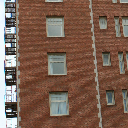
\includegraphics[width = \textwidth]{aliasbrick4.png}
		\caption{$\sigma$ = 0.0}
		\label{fig:aliasbrick4.png}
	\end{subfigure}
	\begin{subfigure}[b]{0.49\textwidth}
		\includegraphics[width = \textwidth]{aabrick75.png}
		\caption{$\sigma$ = 0.75}
		\label{fig:aabrick75.png}
	\end{subfigure}
	\begin{subfigure}[b]{0.49\textwidth}
		\includegraphics[width = \textwidth]{aabrick100.png}
		\caption{$\sigma$ = 1.0}
		\label{fig:aabrick100.png}
	\end{subfigure}
	\begin{subfigure}[b]{0.49\textwidth}
		\includegraphics[width = \textwidth]{aabrick125.png}
		\caption{$\sigma$ = 1.25}
		\label{fig:aabrick125.png}
	\end{subfigure}
\end{figure}
\\
As we can see, the aliasing is almost completely gone when we get to $\sigma$ = 1.25.

\newpage
\subsubsection{Derivative Filters}
I chose to use the sobel filters for this task. I designed them by hand and slapped them into the \emph{imfilter(image, filter)} function.
The magnitude is an approximation, simply adding together the absolute values of the two gradient images. The image I chose was Lena.
The results are as follows:\\

\begin{figure}[h]
	\centering
	\begin{subfigure}[t]{0.49\textwidth}
		\includegraphics[width = \textwidth]{lenadx.png}
		\caption{The $dx$ gradient}
		\label{fig:lenadx.png}
	\end{subfigure}
	\begin{subfigure}[t]{0.49\textwidth}
		\includegraphics[width = \textwidth]{lenady.png}
		\caption{The $dy$ gradient}
		\label{fig:lenady.png}
	\end{subfigure}
	\begin{subfigure}[b]{0.49\textwidth}
		\includegraphics[width = \textwidth]{lenamag.png}
		\caption{The magnitude}
		\label{fig:lenamag.png}
	\end{subfigure}
\end{figure}

Unfortunately, I did not figure out how to display the vector field properly.

\newpage
\subsection{Frequency Domain Filtering}
\subsubsection{Fourier Transform}
To compute and visualize the fourier transform of my images I used these steps:
\begin{lstlisting}
F = fft2(image);
F2 =  fftshift(F);
imshow(log(1+abs(F2)),[0 max]);
\end{lstlisting}
Where max is just above the highest pixel value of the image to be diplayed.


\begin{figure}[h]
	\centering
	\begin{subfigure}[t]{0.45\textwidth}
		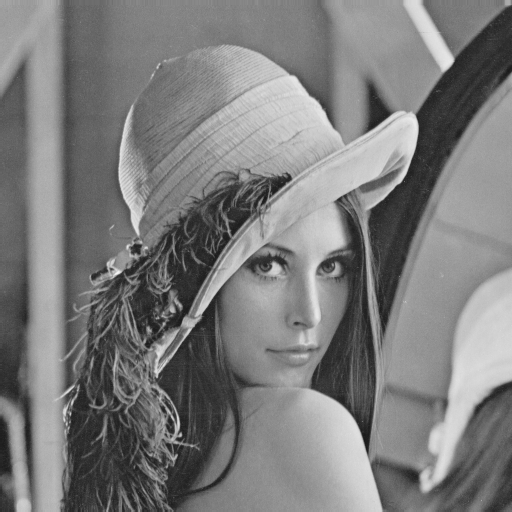
\includegraphics[width = \textwidth]{lena.png}
		\caption{Lena before}
		\label{fig:lena.png}
	\end{subfigure}
	\begin{subfigure}[t]{0.45\textwidth}
		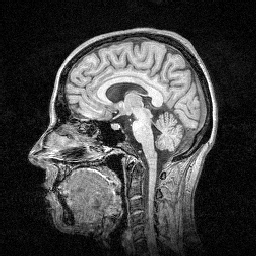
\includegraphics[width = \textwidth]{head.png}
		\caption{Head before}
		\label{fig:head.png}
	\end{subfigure}
	\begin{subfigure}[b]{0.45\textwidth}
		\includegraphics[width = \textwidth]{fftlena.png}
		\caption{Fourier transform of Lena}
		\label{fig:fftlena.png}
	\end{subfigure}
	\begin{subfigure}[b]{0.45\textwidth}
		\includegraphics[width = \textwidth]{ffthead.png}
		\caption{Fourier transform of head}
		\label{fig:ffthead.png}
	\end{subfigure}
\end{figure}

\newpage
\subsubsection{Low- and High pass}
I chose to work with the picture of Lena for this part of the exercise. 

\begin{figure}[h]
	\centering
	\caption{The Filters}
	\begin{subfigure}[t]{0.45\textwidth}
		\includegraphics[width = \textwidth]{lowpass.png}
		\caption{Lowpass filter}
		\label{fig:lowpass.png}
	\end{subfigure}
	\begin{subfigure}[t]{0.45\textwidth}
		\includegraphics[width = \textwidth]{highpass.png}
		\caption{Highpass filter}
		\label{fig:highpass.png}
	\end{subfigure}
\end{figure}

And this is the script used to apply the transformations look like this:
\begin{lstlisting}
function res = fdFilter(image, filter)
    SFT = fftshift(fft2(image));
    filteredSFT = SFT .* filter;
    res = ifft2(ifftshift(filteredSFT));
end
\end{lstlisting}

\newpage
To get a proper result, I had apply the absolute value to my images before viewing.

\begin{figure}[h]
	\caption{The results after filtering}
	\centering
	\begin{subfigure}[t]{0.52\textwidth}
		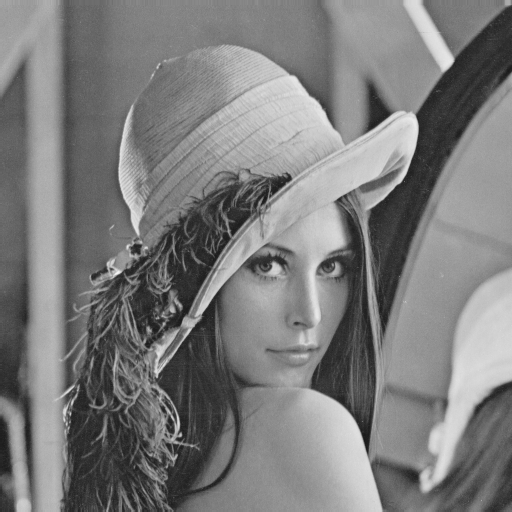
\includegraphics[width = \textwidth]{lena.png}
		\caption{Original}
		\label{fig:lena.png}
	\end{subfigure}
	\begin{subfigure}[b]{0.49\textwidth}
		\includegraphics[width = \textwidth]{lplena.png}
		\caption{Lowpass filtered}
		\label{fig:lplena.png}
	\end{subfigure}
	\begin{subfigure}[b]{0.49\textwidth}
		\includegraphics[width = \textwidth]{hplena.png}
		\caption{Highpass filtered}
		\label{fig:hplena.png}
	\end{subfigure}
\end{figure}

Since my Highpass filter is the inversed lowpass filtered, I end up with a black image if i apply both. This would not happen if the filters were not ideal, or the radiuses of the filters were different. Then I would have a band pass or band reject depending on the radiuses. 

\end{document}

